\chapter{Gráficos con Winston}

\section{Instrucciones básicas}

Vistos algunos de los aspectos básicos del manejo de números, \emph{arrays} y textos, podemos abordar el tema de la representación gráfica de los datos. A menudo, cuando se hace un análisis de datos, lo primero que se desea es visualizarlos en un gráfico. Además, aprender a dibujar gráficos sencillos suele ser más satisfactorio, y da la sensación de poder hacer ``cosas útiles'' desde el principio, más que hacer operaciones numéricas de complejidad equivalente.

La distribución básica de Julia no ofrece utilidades gráficas, pero existen varios paquetes que permiten hacerlas. El más elemental, que utilizaremos aquí, es Winston (\url{https://github.com/nolta/Winston.jl}).%
\footnote{%
Los usuarios de R, y en particular del paquete ggplot2, encontrarán también útil el paquete Gadfly (\url{https://github.com/dcjones/Gadfly.jl}), que permite hacer gráficos mucho más complejos utilizando una sintaxis semejante. Los que tengan Python y su módulo gráfico Matplotlib instalado en el ordenador, también pueden usarlo a través de Julia con el paquete PyPlot (\url{https://github.com/stevengj/PyPlot.jl}).%
}
Recordamos aquí que para instalar este paquete, la forma más sencilla es ejecutar la línea:

\begin{jlconcode}
julia> Pkg.add("Winston")
\end{jlconcode}

Esta operación se hace una sola vez, y al mismo tiempo que Winston, instalará (si no se tienen ya) los distintos paquetes de los que depende. Además, en cada sesión en la que se desee emplear esta herramienta habrá que ``cargar'' el paquete mediante la orden:

\begin{jlconcode}
julia> using Winston
\end{jlconcode}

La función principal es \code{plot}, que se utiliza de manera casi idéntica a la función del mismo nombre en otros lenguajes como Matlab o la biblioteca PyPlot de Python. Partamos de un ejemplo trivial (figura \ref{fig:winston-coseno}):

\begin{jlconcode}
julia> # Dibujar el coseno de x entre 0 y 3pi con 100 puntos
julia> x = linspace(0, 3pi, 100);
julia> y = cos(x);
julia> plot(x, y, "-or")
\end{jlconcode}

\begin{figure}
\centering
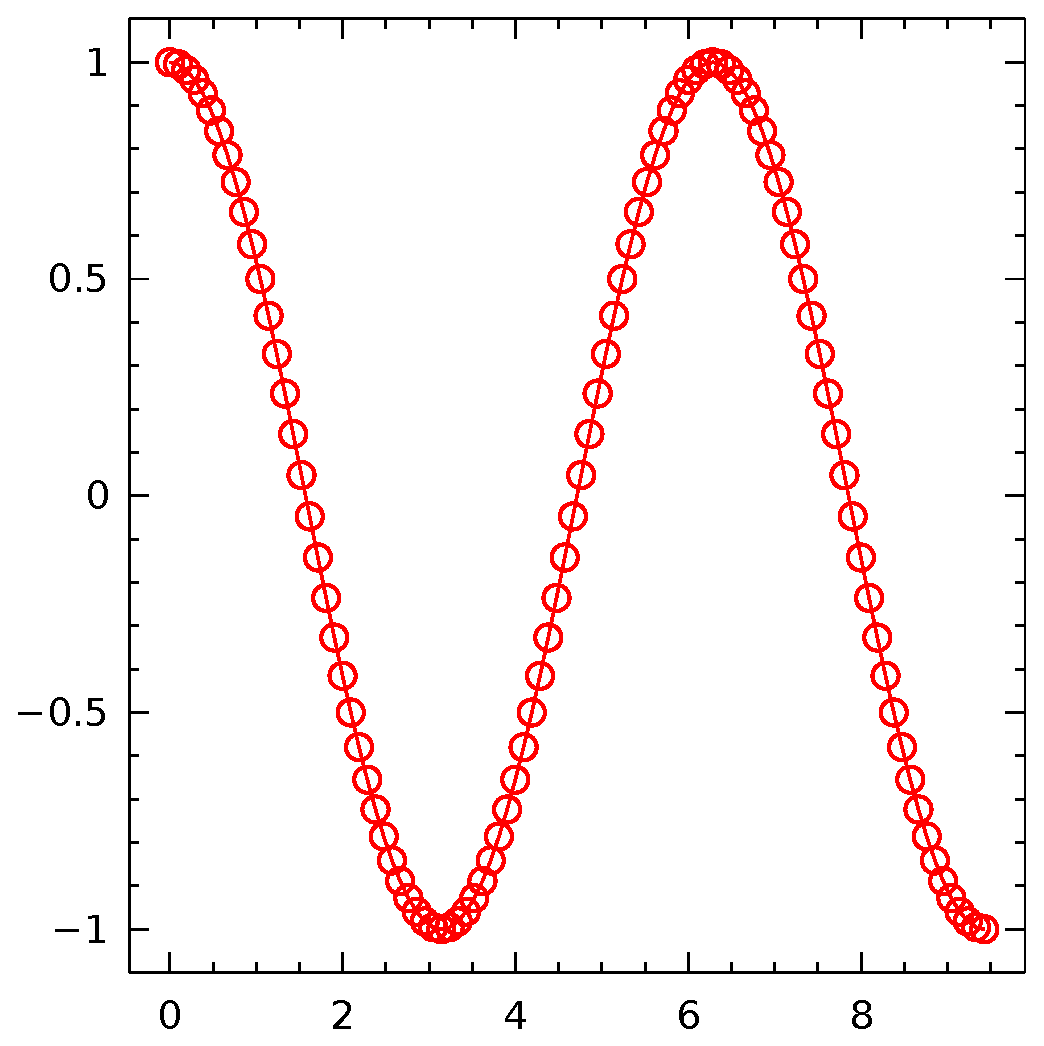
\includegraphics{winston-coseno}
\caption{Ejemplo de gráfico en Winston}
\label{fig:winston-coseno}
\end{figure}

El primer argumento (vector de puntos en el eje $X$) es opcional: si solo se pasa un vector de datos, estos se dispondrán como si el eje $X$ fuese \code{[1:length(y)]}. El tercer argumento (también opcional) es una cadena de texto que indica los atributos gráficos de la serie dibujada (por defecto una linea continua negra). En este caso, una línea continua (\code{'-'}), con puntos marcados como círculos (\code{'o'}), todo ello de color rojo (\code{'r'}). Estos atributos pueden consistir en tipos de linea, marcas de puntos, o colores (figura \ref{fig:winston-modificadores}), y se pueden combinar en cualquier orden, con una excepción: \code{"-."} representa ``linea discontinua alternada con puntos'', mientras que \code{".-"} equivale a ``marcadores en forma de puntos'' + ``linea continua''.

\begin{figure}
\centering
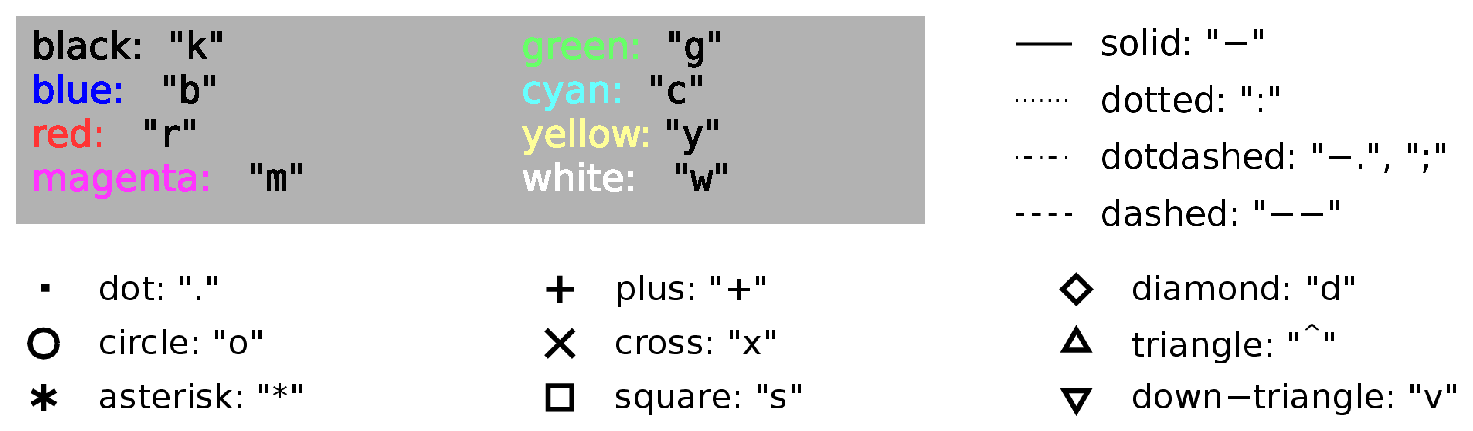
\includegraphics[width=0.8\textwidth]{winston-modificadores}
\caption{Especificaciones de colores, líneas y marcadores}
\label{fig:winston-specs}
\end{figure}


La función \code{plot}, además de representar el gráfico especificado en pantalla, crea en memoria un objeto de la clase \code{FramedPlot} con los contenidos del gráfico, que es el valor devuelto por la función. Es decir, que si hubiéramos escrito, por ejemplo:

\begin{jlconcode}
julia> p = plot(x, y, "-or")
\end{jlconcode}

la variable \code{p} contendría los contenidos del gráfico en cuestión. De este modo, si se cierra la ventana del gráfico o se cambia su contenido, este se puede volver a mostrar invocando a esta variable.

\section{Series de datos superpuestas}

Asignar un gráfico a una variable también sirve para añadirle nuevas series de datos u otros componentes. Si a la función \code{plot} le añadimos un primer argumento con el contenido de un gráfico anterior:

\begin{jlconcode}
julia> # Dibujar sobre el gráfico "p"
julia> plot(p, x, sin(x))
\end{jlconcode}

veremos una nueva linea dibujada sobre la anterior (figura \ref{fig:winston-superposicion}). Si no se hubiera especificado ese primer argumento, simplemente se habría creado un nuevo gráfico que sustituiría al anterior, en lugar de superponerse.

\begin{figure}
\centering
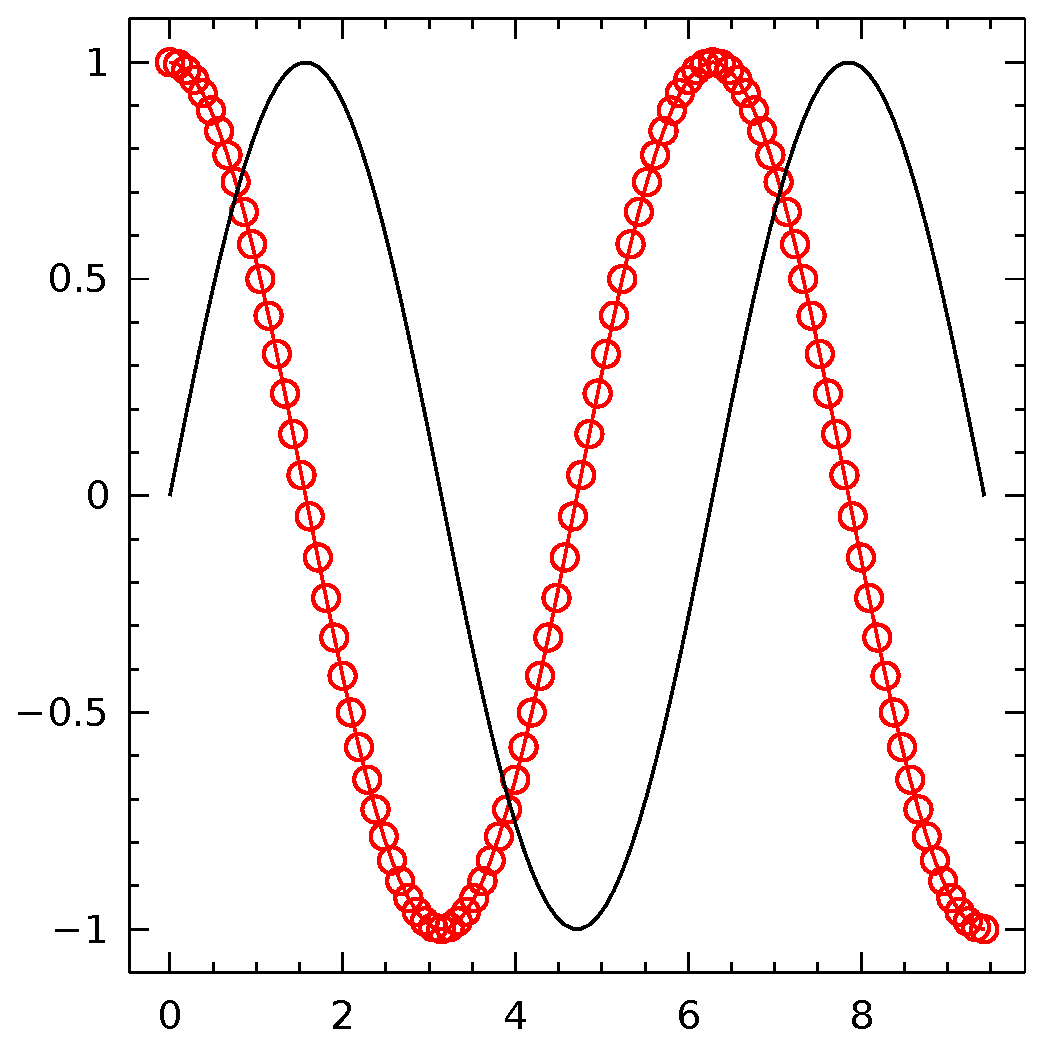
\includegraphics{winston-coseno-seno}
\caption{Superposición de gráficos}
\label{fig:winston-superposicion}
\end{figure}

Esta forma de añadir componentes es especialmente útil si se trabaja con varios gráficos a al vez. Si solo se trabaja con uno, basta con utilizar la función \code{oplot} (forma abreviada de \emph{overplot}), que funciona igual que \code{plot} pero siempre añade la serie de datos especificada al último gráfico que se haya creado.

Otra opción es emplear la función \code{hold}, que altera el comportamiento de \code{plot} en este aspecto:

\begin{jlconcode}
julia> hold(false) # comportamiento por defecto de "plot"
julia> hold(true)  # cambia "plot" para hacer lo mismo que "oplot"
julia> hold()      # alterna ambos comportamientos de "plot"
\end{jlconcode}

Alternativamente, se puede llamar a \code{plot} especificando múltiples series de datos, para que las represente superpuestas en un solo paso.

\begin{jlconcode}
julia> # Esta instrucción también genera el gráfico con dos líneas
julia> plot(x, y, "-or", x, sin(x), "k")
\end{jlconcode}

Como se ve en el ejemplo, los grupos de argumentos (datos en el eje $X$, datos en el eje $Y$, y atributos visuales) se añaden secuencialmente. Los argumentos opcionales (eje $X$ y atributos) se pueden omitir si la secuencia resultante no es ambigua.

Y también hay otra alternativa más sencilla en el caso de que las series de datos tengan la misma longitud: juntar los valores del eje $Y$ en una sola matriz, con cada serie en una columna. La función \code{plot} asigna a cada columna un color distinto por defecto, repitiéndose esta secuencia cada 8 columnas: (1) negro, (2) rojo, (3) verde, (4) azul, (5) naranja, (6) morado/índigo, (7) marrón, (8) violeta/púrpura.

\begin{jlconcode}
julia> # seno en una línea negra, coseno en una línea roja
julia> plot(x, [sin(x) cos(x)])
\end{jlconcode}

\section{Trabajar con múltiples figuras}

Para trabajar con más de un gráfico en pantalla, se deben abrir distintas figuras o ventanas gráficas.%
\footnote{%
Esto es así al menos cuando se trabaja con la interfaz básica de Julia. Los distintos IDEs pueden cambiar la forma de visualizar los gráficos.%
}
Conviene tener clara la diferencia entre los conceptos de ``figura'' y ``gráfico'' (en términos técnicos, \emph{Figure} y \emph{FramedPlot}, respectivamente). El segundo es siempre un contenido de la primera, como se muestra en la figura XXX.

Para crear una nueva figura se utiliza la función \code{figure} sin ningún argumento. Esta función devuelve un número entero que identifica a la figura mientras esta se encuentre abierta. Además hará que esa figura sea la ``activa'', es decir que que desde ese momento todas las operaciones gráficas se hagan sobre ella y sus contenidos.

\begin{jlconcode}
julia> # Crear una nueva figura y asignar su identificador a f
julia> f = figure()
\end{jlconcode}

Si posteriormente se crean otras figuras, se puede volver a activar una anterior, empleando este identificador como argumento de \code{figure}:

\begin{jlconcode}
julia> # f vuelve a ser la figura activa
julia> figure(f)
\end{jlconcode}

La operación complementaria de eliminar una figura creada se lleva a cabo con la función \code{closefig} (aparte de la posibilidad hacer ``click'' sobre el botón para cerrar la figura, cuando se trabaja en modo interactivo):

\begin{jlconcode}
julia> # Cerrar la figura f
julia> closefig(f)
\end{jlconcode}

Es importante mencionar que las figuras recién creadas están ``vacías''; no contienen ningún gráfico, ni siquiera en blanco, hasta que se llama a la función \code{plot} o una equivalente. Esto significa que la función \code{oplot} no actuará sobre ellas. Y tampoco se puede utilizar el identificador de la figura como primer argumento de \code{plot}, ya que se trata de un objeto de distinto tipo. Si se quiere, para crear un gráfico en blanco se puede emplear a la función ``constructora'' \code{FramedPlot}.

Por otro lado, si no hay ninguna figura abierta, las funciones como \code{plot}, \code{FramedPlot}, etc. la crean automáticamente, aunque no dan información sobre ella. Si hace falta, el identificador de la figura activa se puede recuperar con la función \code{gcf} ---sin argumentos---, cuyo nombre representa el acrónimo de \emph{get current figure}.

\begin{jlconcode}
julia> # f identifica a la figura que contiene el gráfico p
julia> p = plot(x, y)
julia> f = gcf()
\end{jlconcode}


\section{Tablas de gráficos, decoraciones y otras complejidades}

Para mostrar de forma práctica otros aspectos de la composición de gráficos, a continuación se plantea un ejemplo algo más complejo, que incluye un par de rutinas habituales: la definición de ``decoraciones'' como títulos, leyendas o etiquetas de los ejes, ajustar el rango de los ejes, y organizar una tabla de gráficos en la misma figura. Este ejemplo también sirve para ver el uso de algunas operaciones rutinarias en cálculos numéricos.

El ejemplo consiste en una composición de dos gráficos (figura \ref{fig:winston-ejemplo-completo}): el gráfico superior muestra una señal de frecuencia modulada y amplitud amortiguada (línea negra), a la que se le ha añadido un error aleatorio (puntos grises), y se ha ajustado con una media ponderada móvil (línea roja). El aspecto más ``ruidoso'' de la señal ajustada en el tramo final se representa en forma de razón entre señal y ruido (\emph{signal-to-noise ratio}, SNR) en el panel inferior. El código para generar este gráfico es el siguiente:

\begin{figure}
\centering
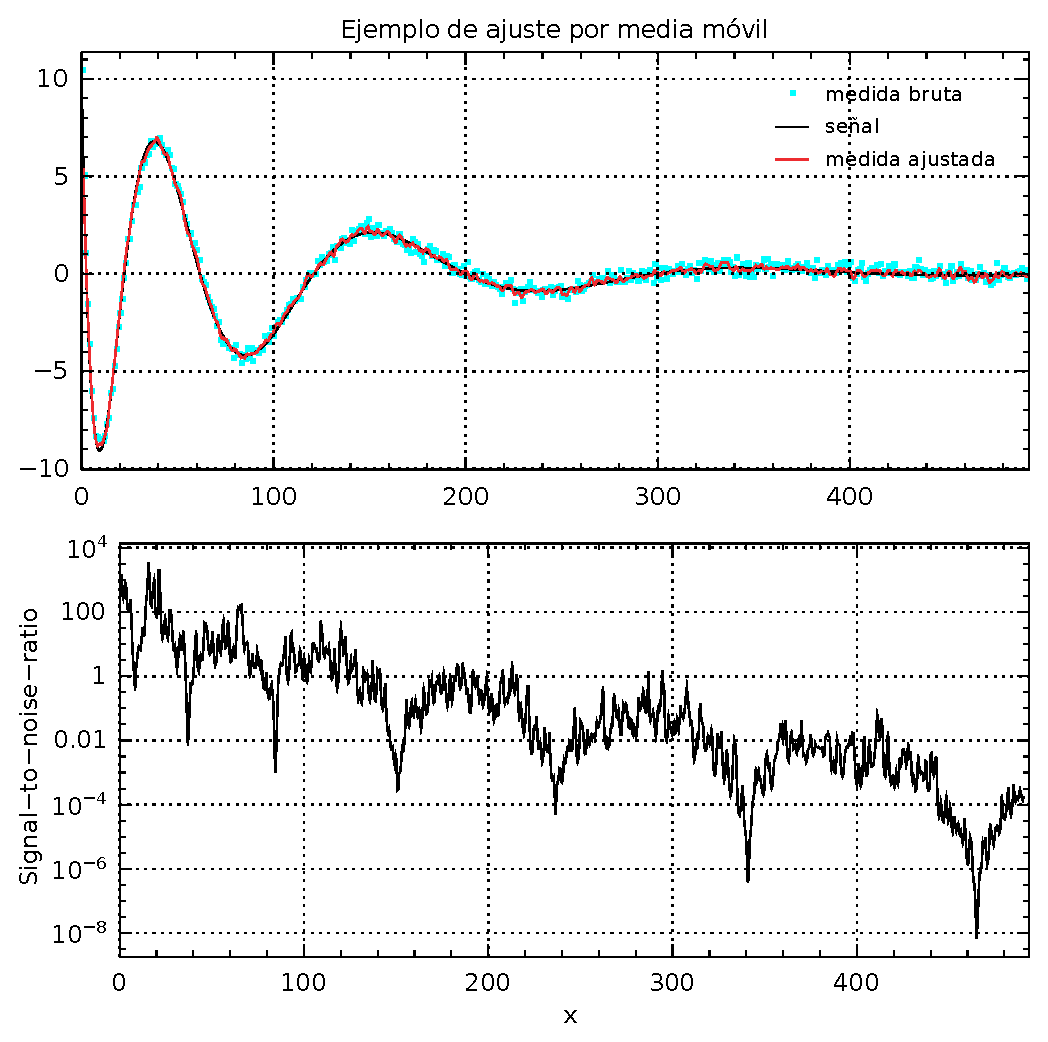
\includegraphics{winston-ejemplo-completo}
\caption{Ejemplo de composición de gráficos}
\label{fig:winston-ejemplo-completo}
\end{figure}

\begin{juliacode}
# x es la variable independiente
x = linspace(0, 50pi^2, 1000)
# f = señal ideal, y = señal observada
f = 10cos(sqrt(x)) .* exp(-x/100)
y = f+0.25randn(1000)
# yfit = señal ajustada con una media ponderada móvil
yfit = fill(NaN, 1000)
b = [1, 2, 3, 2, 1]/9
for t = 3:998
  yfit[t] = sum(y[t-2:t+2] .* b)
end
# Signal-to-noise ratio
# (ver comentario)
signal_pow = fill(NaN, 1000)
noise_pow = fill(NaN, 1000)
noise = yfit - f
for t = 3:998
  signal_pow[t] = sum((f[t-2:t+2] - mean(f[t-2:t+2])).^2)
  noise_pow[t] = sum((noise[t-2:t+2] - mean(noise[t-2:t+2])).^2)
end
snr = (signal_pow./noise_pow)[5:end]
# Aquí empiezan los gráficos
plottable = Table(2, 1)
plottable[1,1] = plot(x[1:2:end], y[1:2:end], ".c", x, [f yfit])
xlim(0,50pi^2)
title("Ejemplo de ajuste por media móvil")
grid(true)
legend(["medida bruta", "señal", "medida ajustada"], 0.75, 0.9)
plottable[2,1] = semilogy(x[3:end-2], snr)
xlim(0,50pi^2)
xlabel("x")
ylabel("Signal-to-noise-ratio")
grid(true)
plottable
savefig(plottable, "figura.png")
\end{juliacode}

Las primeras líneas de este ejemplo son las operaciones realizadas para obtener los datos del panel superior. Se usa la función \code{linspace} para crear un vector de 1000 puntos equiespaciados entre $0$ y $50\pi$, unas sencillas funciones matemáticas para la señal ideal, y la función \code{randn} para añadirle el ruido aleatorio (procedente de una distribución gaussiana).

Este ruido se intenta cancelar con una media ponderada móvil, de ventana triangular de 5 puntos representada por el vector de coeficientes \code{b}. Este último cálculo se realiza con el bucle \code{for}, que es autoexplicativo --- los detalles de esta técnica se presentan en  el siguiente capítulo.%
\footnote{%
Sería mucho más eficiente hacer esta operación con la
función \code{filt}, pero se opta por esta solución más trivial para no
complicar el ejemplo con cuestiones relativas al tratamiento de señales digitales.%
}
Los dos primeros y últimos puntos de la señal ajustada no se calculan, y se dejan como \emph{not-a-numbers} (\code{NaN}), para evitar ``efectos de borde''. Luego se calcula la medida en que varían la señal original y la filtrada para obtener la SNR. Estas variaciones se calculan como una ``suma de cuadrados móvil'' con un ancho de 5 puntos. Esto se hace con un bucle semejante al usado para la media ponderada móvil.

A esto le siguen las operaciones gráficas. Para construir una tabla de gráficos se emplea la función \code{Table} con dos argumentos: el número de filas y columnas de la tabla, respectivamente. El valor devuelto es un objeto del tipo \code{Winston.PlotContainer}. La gráfica creada con la función \code{plot} se asigna al panel que corresponde de esta tabla, del mismo modo que si trabajásemos con \emph{arrays} de datos numéricos.

En este ejemplo, la primera llamada a \code{plot} se utiliza para representar tres series de datos al mismo tiempo. La primera secuencia es la de los puntos observados (\code{".c"} son puntos en color cian), representados de dos en dos para que el gráfico sea menos denso. La segunda secuencia son las dos líneas con la señal original y la ajustada, puestas como un solo conjunto de datos en forma de matriz.

El panel inferior representa la razón entre señal y ruido (\code{snr}), pero en lugar de \code{plot} se utiliza la función \code{semilogy}, porque queremos que el eje Y se represente en escala logarítmica para visualizar mejor cómo varía esta medida. Para poner en escala logarítmica el eje X o ambos, se emplean las funcioines \code{semilogx} y \code{loglog}, respectivamente.

También se muestra el uso de algunas funciones habituales para ajustar los límites del gráfico y ``decorar'' el contexto. (véase que estas funciones se han llamado tras crear los objetos gráficos del panel que se quiere modificar):

\begin{itemize}
  \item \code{xlim} define los límites inferior y superior del eje $X$ (el eje $Y$ se ajusta con \code{ylim})
  \item Las funciones \code{title}, \code{xlabel}, \code{ylabel} sirven para añadir texto al título y los dos ejes, respectivamente
  \item \code{grid} se emplea para añadir o eliminar la cuadrícula en el area gráfica
  \item \code{legend} añade una leyenda con los textos especificados para las distintas series de datos representadas; el primer argumento es un vector de cadenas de texto, ordenadas según se han creado los elementos gráficos que se etiquetan en la leyenda; los dos siguientes argumentos son las coordenadas de la ``caja'' que contiene la leyenda, relativas al área de la figura ($(0,0)$ representa la esquina inferior izquierda, y $(1,1)$ la superior derecha).
\end{itemize}

Hacia el final se llama a la tabla de gráficos por su nombre, para mostrar el resultado una vez terminado el proceso. El motivo es que si las líneas del código se ejecutan una a una en modo interactivo, se verá que al llamar a la función \code{Table} aparece una figura en blanco; luego, cuando se crea cada uno de los gráficos, estos sustituyen a la figura vacía ocupando toda la ventana gráfica. La tabla con los dos gráficos combinados solo aparece al volver a llamar a la tabla de gráficos al final. Este comportamiento recalca la importancia de asignar el objeto devuelto por \code{Table} a una variable, ya que para visualizar la tabla de gráficos hay que llamarla explícitamente después de crearla. Ni siquiera ocultando los dos gráficos individuales (por ejemplo añadiendo un punto y coma tras las líneas segunda y tercera) se hubiera actualizado la vista de la tabla, hasta llamar la última línea.

Finalmente, para salvar el resultado a un archivo gráfico, basta con darle el nombre del archivo a la función \code{savefig}. Los tipos de archivo soportados por la función son EPS, PDF, SVG y PNG. El identificador del gráfico es opcional ---por defecto se imprime el gráfico de la figura activa---, y en el caso de guardarse un archivo de tipo PDF, se puede asignar un vector de gráficos (objetos de tipo \code{PlotContainer}), cada uno de los cuales se imprimirá en una página distinta.


\section{Edición de gráficos}

De vez en cuando se desea cambiar algún atributo de las gráficas creadas, lo cual puede conseguirse habitualmente con las funciones \code{setattr} y \code{style}.

Su uso se muestra algunos ejemplos que pueden ser más o menos habituales, siguiendo con el caso mostrado en la sección anterior. La lista completa de atributos asignados a cada tipo de objeto se puede encontrar en la referencia del paquete Winston (\url{https://github.com/nolta/Winston.jl/wiki/Reference}), así como otros ejemplos en \url{http://winston.readthedocs.org/}. También se pueden visualizar la estructura de un gráfico, incluyendo sus atributos, con la función \code{dump}:

\begin{jlconcode}
julia> dump(plottable[1,1])
Winston.FramedPlot 
  attr: Dict{Any,Any} len 6
    title_offset: Float64 1.0
    page_margin: Float64 0.1
    gutter: Float64 0.1
    aspect_ratio: Void nothing
    title: UTF8String "Ejemplo de ajuste por media móvil"
    title_style: Dict{Symbol,Any} len 1
      fontsize: Float64 3.0
  content1: Winston.PlotComposite 
    attr: Dict{Any,Any} len 1
      style: Dict{Symbol,Any} len 0
    components: Array(Any,(4,))
      1: Winston.Points 
        attr: Dict{Any,Any} len 2
          style: Dict{Symbol,Any} len 3
          label: UTF8String "medida bruta"
        x: LinSpace{Float64} 
          start: Float64 0.0
          stop: Float64 492.9862458602192
          len: Float64 500.0
          divisor: Float64 499.0

[Output truncado]
\end{jlconcode}

En el fragmento mostrado se ven los 6 atributos del panel superior, del que el más obvio es el título (\code{title}). Por lo tanto, si se quisiera editar el título en cualquier momento (por ejemplo para ponerlo en mayúsculas):

\begin{jlconcode}
julia> # Con getattr se obtiene el valor actual del atributo
julia> titulo = getattr(plottable[1,1], "title")
"Ejemplo de ajuste  media móvil"
julia> # Lo convertimos en mayúscula, y lo reasignamos con setattr
julia> # usando el argumento con el nombre correspondiente
julia> setattr(plottable[1,1], title=uppercase(titulo))
julia> # Volvemos a llamar al gráfico para que se vea el resultado
julia> plottable
\end{jlconcode}

También se pueden ver las series de datos representadas por los objetos dentro del vector \code{components} en el campo \code{content1} (en el fragmento mostrado se ven las primeras líneas referidas a la serie de puntos).%
\footnote{%
Todo gráfico tiene sus contenidos distribuidos en \code{content1} y
\code{content2}. En los más habituales todo se encuentra dentro de
\code{content1}.%
}
El conjunto de componentes se puede extraer con la función \code{getcomponents}, para facilitar su edición.

\begin{jlconcode}
julia> comp = getcomponents(plottable[1,1])
4-element Array{Any,1}:
 Winston.Points(...)
 Winston.Curve(...) 
 Winston.Curve(...) 
 Winston.Legend(...)
\end{jlconcode}

Las propiedades visuales de las series de datos, como el tipo y color de las líneas y los puntos, están en un atributo especial llamado \code{style} (estilo):

\begin{jlconcode}
julia> # Atributos del primer componente (serie de puntos)
julia> # El campo "attr" del objeto "xxx" se extrae como "xxx.attr"
julia> dump(comp[1].attr)
Dict{Any,Any} len 2
  style: Dict{Symbol,Any} len 3
    symbolkind: ASCIIString "dot"
    color: ColorTypes.RGB{FixedPointNumbers.UFixed{UInt8,8}} 
      r: FixedPointNumbers.UFixed{UInt8,8} 
        i: UInt8 0
      g: FixedPointNumbers.UFixed{UInt8,8} 
        i: UInt8 255
      b: FixedPointNumbers.UFixed{UInt8,8} 
        i: UInt8 255
    symbolsize: Float64 1.0
  label: UTF8String "medida bruta"

julia> # Lo mismo para las dos líneas
julia> dump(comp[2].attr)
Dict{Any,Any} len 3
  style: Dict{Symbol,Any} len 2
    linecolor: UInt32 0
    linewidth: Float64 2.0
  label: UTF8String "señal"
  kw_defaults: Dict{Symbol,Any} len 1
    linewidth: Float64 2.0

julia> dump(comp[3].attr)
Dict{Any,Any} len 3
  style: Dict{Symbol,Any} len 2
    linecolor: UInt32 15543344
    linewidth: Float64 2.0
  label: UTF8String "medida ajustada"
  kw_defaults: Dict{Symbol,Any} len 1
    linewidth: Float64 2.0
\end{jlconcode}

Supongamos que para resaltar los aspectos de interés, queremos convertir el color de los puntos a gris, presentar la señal ideal como una línea roja discontinua gruesa, y la medida ajustada como una línea azul más delgada (figura \ref{fig:winston-ejemplo-modificado}). Para ello utilizaremos las siguientes instrucciones:

\begin{jlconcode}
julia> style(comp[1], color="grey")
julia> style(comp[2], linekind="dashed", linecolor="red", linewidth=3)
julia> style(comp[3], linewidth=1.5, linecolor="blue")
julia> plottable
\end{jlconcode}

\begin{figure}
\centering
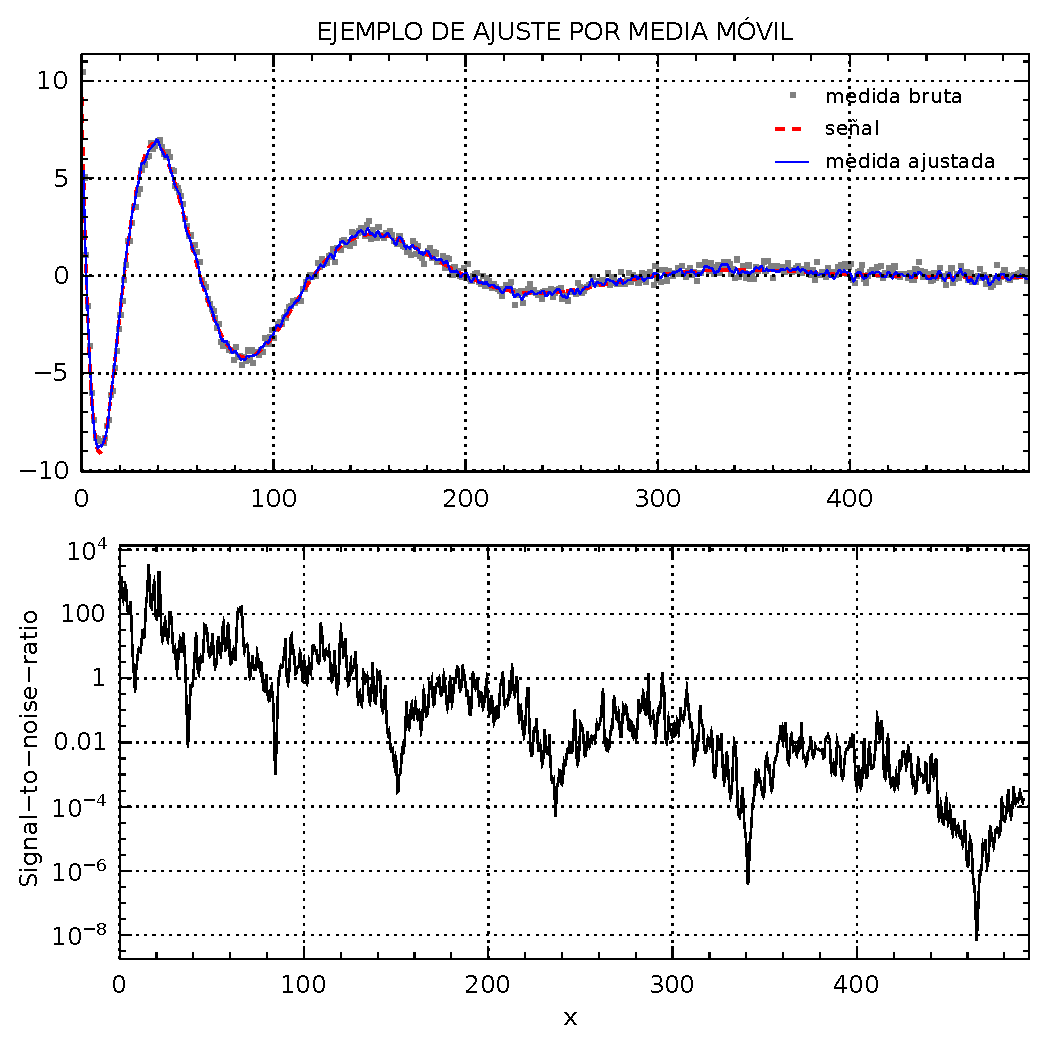
\includegraphics{winston-ejemplo-modificado}
\caption{Superposición de gráficos}
\label{fig:winston-ejemplo-modificado}
\end{figure}

\section{Otros gráficos}

La función \code{plot} es la más habitual para representar series de datos, pero también hay más funciones para otro tipo de representaciones, entre otras:

\begin{itemize}
  \item \code{stem}: gráficos de ``tallos''. Representan series de datos, al igual que \code{plot}, pero se añaden líneas verticales que conectan cada punto con el eje $Y=0$.
  \item \code{scatter}: gráficos de dispersión. Se diferencia de \code{plot} en que es necesario especificar los valores en el eje $X$, por defecto se representan puntos, no líneas, y también se pueden introducir variables que especifican el tipo y el color de cada punto individual.
  \item \code{errorbar}: barras de error. A los valores del eje $X$ e $Y$ se les añade el argumento \code{xerr} o \code{yerr}, según si se quieren representar barras horizontales o verticales, respectivamente. Este argumento ha de escribirse con el nombre explícito, para evitar ambigüedades. Si la serie de datos contiene $n$ puntos, este argumento ha de ser un vector numérico de longitud $n$ (para barras simétricas) o $2n$ (para especificar distintas amplitudes en ambas direcciones a partir de los puntos especificados). En este último caso, los valores de $1$ a $n$ del argumento adicional representa cuánto se extiende la barra hacia la izquierda (para \code{xerr}) o hacia abajo (para \code{yerr}), y del $n+1$ hasta el $2n$ cuánto se extiende hacia la derecha o hacia arriba, respectivamente.
  %\item \code{bar}, \code{barh}: diagramas de barras verticales y horizontales, respectivamente. El primer argumento especifica las etiquetas que se presentan en los valores del eje $X$ ($Y$ para las barras horizontales). El segundo representa las alturas de cada barra; si es una matriz $N\times{}M$, se presentan $N$ grupos de $M$ barras coloreadas.
  \item \code{plothist}: histogramas. Se le pasa un vector de datos, e internamente usa la función \code{hist} para definir los intervalos del eje $X$ y calcular las frecuencias del vector en esos intervalos. Como en esa función, se puede definir el número (aproximado) de barras o los límites exactos de las mismas añadiendo dichos valores como argumentos adicionales.
  \item\code{hist2d}: histograma bidimensional. En este caso se le pasa una matriz de dos columnas, y los ejes $X$, $Y$ de la imagen se asocian a los intervalos de la primera y la segunda columna, respectivamente. Las frecuencias para cada combinación de intervalos se representan en una escala de color.
  \item\code{imagesc}: mapas de color a partir de una matriz de datos. Los argumentos requeridos son, en orden: el intervalo en el eje $X$, el intervalo en el eje $Y$, la matriz de datos a representar ($X$ en filas, $Y$ en columnnas), y el intervalo de valores de la matriz al que se ajusta la escala de colores. El único argumento requerido es la matriz de datos, y los omitidos se calculan automáticamente.
\end{itemize}

Las funciones \code{hist2d} o \code{imagesc} utilizan ``mapa de color'' para representar los datos. Por defecto el mapa empleado es el llamado \emph{jet} o ``arcoiris''. Este mapa de colores se puede cambiar por una escala de degradados de distintos colores, a través de la función \code{colormap} --- que se ha de llamar \emph{antes} de crear el gráfico:

\begin{juliacode}
colormap("blues")   # Escala de azules
colormap("greens")  # Escala de verdes
colormap("grays")   # Escala de grises
colormap("oranges") # Escala de naranjas
colormap("purples") # Escala de púrpuras
colormap("reds")    # Escala de rojos
\end{juliacode}
